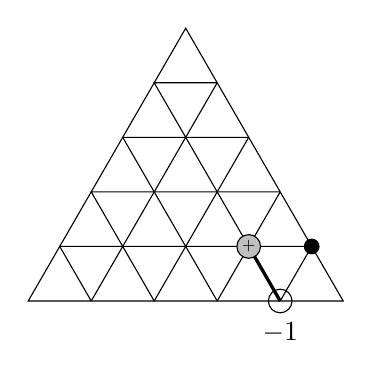
\begin{tikzpicture}[baseline=0cm]
\draw (0,0) -- (4,0) -- (60:4) -- cycle;

\foreach \x in {0.8,1.6,2.4,3.2}
\draw (4,0)++(120:\x) edge (4-\x,0) -- (60:\x) -- (\x,0);

\fill (4,0) ++(120:0.8) circle[radius=0.1];% ++(0,-0.4)node{$v$};
\draw[very thick] (3.2,0) ++(120:0.8) -- (3.2,0);
\draw (3.2,0) circle[radius=0.15] ++(0,-0.4)node{$-1$};

\draw[fill=lightgray] (4,0) ++(120:0.8)
	++(180:0.8)node{\tiny$+$} circle[radius=0.15];
\end{tikzpicture}